\documentclass[twoside]{article}

\usepackage{ustj}

\usepackage{tikz}
\newcommand{\bit}[1]{%
  \tikz[baseline=(char.base)]{%
    \node[shape=rectangle, draw, rounded corners=1pt, inner sep=1pt, minimum width=6pt, minimum height=6pt] (char) {#1};
  }%
}

\setcounter{tocdepth}{2}

\addbibresource{mss.bib}

\newcommand{\authorname}{N. E. Davis, Brian Klatt, \& Sam Parker}
\newcommand{\authorpatp}{\patp{lagrev-nocfep}, \patp{zod}, \& \patp{zod}}
\newcommand{\affiliation}{Zorp Corp, Zorp Corp, \& —}

%  Make first page footer:
\fancypagestyle{firststyle}{%
\fancyhf{}% Clear header/footer
\fancyhead{}
\fancyfoot[L]{{\footnotesize
              %% We toggle between these:
              Manuscript submitted for review.\\
              % {\it Urbit Systems Technical Journal} II:2 (2025):  1–46. \\
              % ~ \\
              % Address author correspondence to \authorpatp.
              }}
}
%  Arrange subsequent pages:
\fancyhf{}
\fancyhead[LE]{{\urbitfont Urbit Systems Technical Journal}}
\fancyhead[RO]{Serializing Nouns}
\fancyfoot[LE,RO]{\thepage}

%%MANUSCRIPT
\title{Serializing Nouns}
\author{N.\ E.\ Davis \patp{lagrev-nocfep}, Brian Klatt \patp{zod},\thanks{Brian Klatt contributed the description of \texttt{++jam}.} \\ \& Sam Parker \patp{zod}\thanks{Sam Parker contributed the description of \texttt{++bulk}.} \\ \affiliation}
% TODO Brian Klatt credit
\date{}

\begin{document}

\maketitle
\thispagestyle{firststyle}

\begin{abstract}
Noun serialization is commonly used for Nock communication, both between instances like Urbit ships and with the runtime and the Unix host operating system.  This article describes and compares the two principal conventions for representing nouns in slightly compressed form as byte arrays, as well as introduces variant encodings for educational purposes.
\end{abstract}

% We will adjust page numbering in final editing.
\pagenumbering{arabic}
\setcounter{page}{1}

\tableofcontents

\section{Introduction}

The Nock combinator calculus deals in nouns and does not know about bit encodings or memory layouts.  A Nock interpreter (runtime) must, however, deal with the practicalities.  In other words, there must be a way of writing down an abstract binary tree (consisting of cells/pairs and atoms) as an actual, physical array of bits in memory.  Every possible Nock noun can be represented as a finite sequence of bytes (an atom), and there are multiple ways to do so.\footnote{The converse is not true:  not every atom represents a valid deserialization or conversion from a graph encoding.}

A noun serialization strategy is rather like a Gödel numbering in that it systematically encodes a mathematical object (a noun) as a number (an atom).  Unlike Gödel numbering, which classically serially encodes the symbols of mathematical statements, noun serialization encodes a binary tree structure.\footnote{This also echoes the way that S-expressions are encoded in Lisp.}  Because a noun may be any atom---and atoms cannot have leading zeroes---both structure and value need to be unambiguously encoded and cannot be simply delimited (as by a \texttt{0} bit or similar).  There are two basic strategies to encode a noun as an atom:

\begin{enumerate}
  \item  Run-length serialization, with or without references.
  \item  Directed graph serialization, depending on a reentrant graph encoding.
\end{enumerate}

\noindent
Both of these embody a tradeoff between simplicity, size, and speed.  Below, we describe both of these strategies and some new variants which offer possible advantages.  Reversible noun encoding is essential for Nock communication, both between Nock execution layers such as Vere and NockVM, and between the runtime and the host operating system.

\section{Na\"{i}ve Serialization}

A noun may be an atom or a cell, and so we first propose to label nodes by type, with \texttt{0} for atom and \texttt{1} for cell.

\begin{figure}[ht]
\centering
\begin{subfigure}
\centering
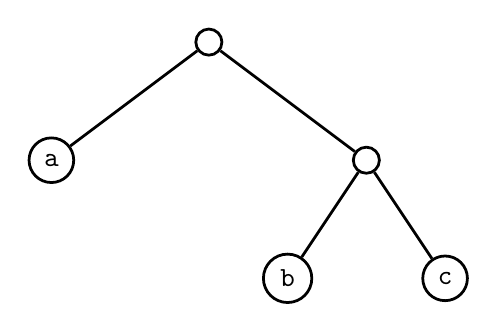
\begin{tikzpicture}[
  level 1/.style={sibling distance=40mm, line width=1pt},
  level 2/.style={sibling distance=20mm, line width=1pt},
  every node/.style={circle,draw, line width=1pt}
  ]
  \node {}
    child { node {\texttt{a}} }
    child { node {}
      child { node {\texttt{b}} }
      child { node {\texttt{c}} }
    };
\end{tikzpicture}
\end{subfigure}
\begin{subfigure}
\centering
\begin{tikzpicture}[
  level 1/.style={sibling distance=40mm, line width=1pt},
  level 2/.style={sibling distance=20mm, line width=1pt},
  every node/.style={square,draw, line width=1pt}
  ]
  \node {1}
    child { node {0} }
    child { node {1}
      child { node {0} }
      child { node {0} }
    };
\end{tikzpicture}
\end{subfigure}
\caption{The noun \texttt{[a b c]} (the same as \texttt{[a [b c]]}) as a binary tree and its metadata labeling in the simplest scheme.}
\label{fig:binary-tree}
\end{figure}

\noindent
The noun in Figure~\ref{fig:binary-tree} is represented as a binary tree, where each node is labeled with its type (atom or cell) and its value (if applicable).  To serialize this noun, we can perform a pre-order traversal of the tree, recording the type and value of each node.  The serialized form would be (in \textsc{lsb} order):

\begin{lstlisting}[style=listingcode]
c 0 b 0 1 a 0 1
\end{lstlisting}

\noindent
The issue, however, is that in decoding this bitstream we do not know where an atom value (such as \texttt{a}) ends.  After all, the point of serialization is to be able to deserialize the bitstream back into the original noun.  Thus we need a way to indicate the length of each atom.

Let's augment this scheme by providing length information for each atom.  One basic idea is to include a string of \texttt{0} bits as the least-significant bits (\textsc{lsb}) of the atom which indicates the length of the atom in bits.  Since the atom could be zero, we also delimit the length with a \texttt{1} bit.  (See Table~\ref{tab:atom-encodings} for examples.)

$$
a = a_{\ell-1} a_{\ell-2} \ldots a_{1} a_{0}
\xrightarrow[\textrm{encode}]{}
\bar{a} = a_{\ell-1} a_{\ell-2} \ldots a_{1} a_{0} \; \mathtt{1} \; \mathtt{0}^{n}
\textrm{,}
$$

\noindent
where $\bar{a}$ is the encoded atom $a$ and $a$ has length $\ell$ bits.\footnote{We will use the overbar notation $\bar{a}$ throughout to notionally indicate the encoded form of $a$, regardless of the method used.}

\begin{table}[ht]
\centering
\caption{Example atom encodings with length information appended as trailing zeros.}
\label{tab:atom-encodings}
\begin{tabular}{ l l r }
  \textbf{Atom} & \textbf{Length (bits)} & \multicolumn{1}{l}{\textbf{Encoded Form}} \\
  \hline
  \texttt{0b0} & 1 & \texttt{0b010} \\
  \texttt{0b1} & 1 & \texttt{0b110} \\
  \texttt{0b10} & 2 & \texttt{0b10100} \\
  \texttt{0b11} & 2 & \texttt{0b11100} \\
  \texttt{0b101} & 3 & \texttt{0b1011000} \\
  \texttt{0b111} & 3 & \texttt{0b1111000} \\
  \texttt{0x70} & 7 & \texttt{0b111000010000000} \\
  \texttt{0xff} & 8 & \texttt{0b11111111100000000} \\
\end{tabular}
\end{table}

For instance, the atom \texttt{0b101010} (decimal \texttt{42}) could be encoded as:

\begin{lstlisting}[style=listingcode]
:: atom 0x2a
> `@ub`(gel 0b101010)
0b101010
:: cell [0x2a 0x3b]
> `@ub`(gel [0b101010 0b111011])
0b1.101010@0.111011
\end{lstlisting}


The simplest way to encode a noun as a binary tree in an atom (byte array) without compression is to utilize bits to mark atom (\texttt{0}) vs. cell (\texttt{1}), the length of the atom in unary of \texttt{1}s terminated by \texttt{0}, and the actual value.  (Since the leading zeros are stripped, they may need to be added back in.)  This is in least-significant \emph{byte} (\textsc{lsb}) order, so you should read the written atom starting from the \emph{right} in binary.

Thus the atom \texttt{0b0} would simply be encoded as:

\begin{lstlisting}[style=listingcode]
:: 0x0 = 0 for atom; 1 for length (special case);
::       0 for end of length; 0 for value
> `@ub`(gel 0b0)
0b10
\end{lstlisting}

\noindent
interpreted as (rightmost, LSB) \texttt{0} for atom, run length of \texttt{1}, and value \texttt{0} (stripped).  I.e., \texttt{0b010} or

{
\centering
$\leftarrow$ \\
\bit{0} \bit{1} \bit{0}
}

Other values include:

\begin{lstlisting}[style=listingcode]
:: 0x1 = 0 for atom; 1 for length;
::       0 for end of length; 1 for value
> `@ub`(gel 0b1)
0b1010

:: [0x0 0x1] = 1 for cell; zero, then one
> `@ub`(gel [@0b0@ 0b1])
0b1.010@0.010@1

:: [0x1 0x0] = 1 for cell; one, then zero
> `@ub`(gel [@0b0@ 0b1])
0b10@1.010@1

:: 0x2 = 0 for atom; 2 for length;
::       0 for end of length; 2 for value
> `@ub`(gel 0b10)
0b10.0111

:: 0xff
> `@ub`(gel 0xff)
0b11.1111.1101.1111.1110

:: [[0x0 0x1] [0x2 0x3]]
> `@ub`(gel [@0b0@ 0b1])
0b10@1.010@1
\end{lstlisting}

Our code implementation for \texttt{++gel} is as follows:

\begin{lstlisting}[style=listingcode]
!:  |%
++  gel
  =gel !:  |=  a=*
  ^-  @
  =+  l=0
  =+  b=0
  =<  -
  |-
  ?^  a
    =+  lv=$(a -.a)
    =+  rv=$(a +.a)
    =+  [c l]=(mash rv lv)
    [(con (lsh [0 1] c) 0b1) +(l)]
  ?:  =(0 a)  [0b10 4]
  :: need another mash in here for unary length
  =+  [c l]=(mash [a l] [b +((met 0 b))])
  [(con (lsh [0 1] c) 0b0) +(l)]
:: length of atom in unary
++  len
  |=  a=@
  ^-  @
  (fil 0 (met 0 a) 0b1)
:: mash two atoms together
++  mash
  |=  [a=[p=@ l=@] b=[p=@ l=@]]
  ^-  [c=@ l=@]
  :-  (con (lsh [0 l.b] p.a) p.b)
  (add l.a l.b)
--
\end{lstlisting}

Note that \texttt{l} is not the length of an atom in unary, but the length of the encoded noun in binary.

\section{Practical Serialization}

Whatever the pedagogical advantages of \texttt{++gel}, the algorithm has practical flaws:  it is subject to collisions XXX
and it is verbose.\footnote{Note the claim of \patp{dozreg-toplud}, p.~TODO of this issue, that an operational Arvo instance may have up to $1.66 \times 10^{21}$ nouns, greatly reduced by structural sharing.}  \texttt{++jam} improves the basic strategy by altering the \textsc{rle} algorithm slightly and supporting internal references for noun subtrees that have already been encoded.

\texttt{++jam} converts a noun into a buffer and deduplicates repeated subtrees.  It walks subtrees and encodes each in a way that allows for efficient storage and retrieval, while also permitting references to previously encoded values.

- get Bryan notes

special-cases 0

The new \textsc{rle} calculation is to post the number plus one in binary rather than unary (e.g., for \texttt{} the length would be \texttt{0b010}).

(Since there is a value less significant than the length, the leading zero is not lost but serves as a divider.)

\begin{lstlisting}[style=listingcode]
++  jam
  ~/  %jam
  |=  a=*
  ^-  @
  =+  b=0
  =+  m=`(map * @)`~
  =<  q
  |-  ^-  [p=@ q=@ r=(map * @)]
  =+  c=(~(get by m) a)
  ?~  c
    =>  .(m (~(put by m) a b))
    ?:  ?=(@ a)
      =+  d=(mat a)
      [(add 1 p.d) (lsh 0 q.d) m]
    =>  .(b (add 2 b))
    =+  d=$(a -.a)
    =+  e=$(a +.a, b (add b p.d), m r.d)
    :+  (add 2 (add p.d p.e))
      (mix 1 (lsh [0 2] (cat 0 q.d q.e)))
    r.e
  ?:  ?&(?=(@ a) (lte (met 0 a) (met 0 u.c)))
    =+  d=(mat a)
    [(add 1 p.d) (lsh 0 q.d) m]
  =+  d=(mat u.c)
  [(add 2 p.d) (mix 3 (lsh [0 2] q.d)) m]
\end{lstlisting}

A Python example of \texttt{++jam} is included in Appendix~A.

\subsection{\texttt{newt} Encoding}

\sloppy
“Newt” encoding is a runtime-oriented extension of \texttt{++jam}\-based noun serialization which adds a short identifying header in case of future changes to the serialization format.  A \mbox{version} number (currently a single bit) precedes a \textsc{rle} serialization length followed by the \texttt{++jam} serialization of the noun.  The version number is currently \texttt{0b0}.

\begin{lstlisting}[style=listingcode]
  V.LLLL.JJJJ.JJJJ.JJJJ.JJJJ.JJJJ.JJJJ
\end{lstlisting}

\noindent
where \texttt{V} is the version number, \texttt{L} is the total length of the noun in bytes, and \texttt{J} is the \texttt{++jam} serialization of the noun.

Runtime communications vanes like \texttt{\%khan} and \texttt{\%lick} utilize this encoding locally.  It is exclusively used as a host OS runtime affordance at the current time.

\section{Directed Graph Encoding}

A directed graph encoding has been independently proposed twice, once by Tlon in the original Hoon codebase as a \lstinline[style=inlinecode]{+$silo} encoding and once by Sam Parker as the \lstinline[style=inlinecode]{++bulk} encoding.


\section{Aligned Serialization}

One of the advantages of \texttt{++jam} is its compactness.  However, this comes at the cost of speed, since bit-level operations are required to \texttt{++cue} the noun back from its serialized form.  If a slightly larger size is acceptable, a byte-aligned serialization could facilitate certain kinds of external inspection without requiring deserialization.  (For instance, a byte-aligned head tag could be read for a rapid decision without needing to \texttt{++cue} the entire noun.)

We propose a strategy to modify \texttt{++jam} to align to bytes by padding the length of entries to the nearest byte boundary and marking the distance with a clever binary scheme rather than simply unary.  This approach, called \texttt{++honey}, aims to balance compactness and speed for certain use cases while retaining a large degree of conceptual backwards compatibility.  (The change in byte alignment of course breaks strict compatibility.)

There are two fundamental issues for byte alignment:  atoms and lengths.  Atoms can be padded with leading zeros to the nearest byte boundary without changing their value.  Lengths, however, require a new encoding scheme to compensate for the adjustment in expected bit widths.  %We propose a variable-length encoding for lengths that uses the high bit of each byte to indicate whether more bytes follow.  The remaining seven bits of each byte contribute to the length value.  This allows for efficient representation of lengths while maintaining byte alignment.

\section{Benchmarks}

\section{Conclusion}

\section*{Appendix A:  Python \texttt{++jam}/\texttt{++cue}}

The following is a simple Python implementation of \texttt{++jam} serialization drawn from Urbit’s auxiliary \texttt{pynoun} library.

\begin{lstlisting}[style=listingcode_python]
from bitstring import BitArray
noun = int | Cell
# The Cell class represents an ordered pair of two nouns.

def jam_to_stream(n: noun, out: BitArray):
    """jam but put the bits into a stream

    >>> s = BitArray()
    >>> jam_to_stream(Cell(0,0), s)
    >>> s
    BitArray('0b100101')
    """

    cur = 0
    refs = {}

    def bit(b: bool):
        nonlocal cur
        out.append([b])
        cur += 1

    def zero():
        bit(False)

    def one():
        bit(True)

    def bits(num: int, count: int):
        nonlocal cur
        for i in range(0, count):
            out.append([(num & (1 << i)) != 0])
        cur += count

    def save(a: noun):
        refs[a] = cur

    def mat(i: int):
        if 0 == i:
            one()
        else:
            a = i.bit_length()
            b = a.bit_length()
            above = b + 1
            below = b - 1
            bits(1 << b, above)
            bits(a & ((1 << below) - 1), below)
            bits(i, a)

    def back(ref: int):
        one()
        one()
        mat(ref)

    def r(a: noun):
        dupe = refs.get(a)
        if deep(a):
            if dupe:
                back(dupe)
            else:
                save(a)
                one()
                zero()
                r(a.head)
                r(a.tail)
        elif dupe:
            isize = a.bit_length()
            dsize = dupe.bit_length()
            if isize < dsize:
                zero()
                mat(a)
            else:
                back(dupe)
        else:
            save(a)
            zero()
            mat(a)
    r(n)

def jam(n: noun):
    """urbit serialization: * -> @

    >>> jam(0)
    2
    >>> jam(Cell(0,0))
    41
    >>> jam(Cell(Cell(1234567890987654321, \\
    ...               1234567890987654321), \\
    ...          Cell(1234567890987654321, \\
    ...               1234567890987654321)))
    22840095095806892874257389573
    """

    out = BitArray()
    jam_to_stream(n, out)
    return read_int(len(out), out)

def cue_from_stream(s: BitArray):
    """cue but read the bits from a stream

    >>> s = BitArray('0b01')
    >>> cue_from_stream(s)
    0
    """

    refs = {}
    cur = 0
    position = 0

    def bits(n: int):
        nonlocal cur, position
        cur += n
        result = 0
        for i in range(n):
            result |= (1 if s[position] else 0) << i
            position += 1
        return result

    def one():
        nonlocal cur, position
        cur += 1
        bit = s[position]
        position += 1
        return bit
    
    def rub():
        z = 0
        while not one():
            z += 1
        if 0 == z:
            return 0
        below = z - 1
        lbits = bits(below)
        bex = 1 << below
        return bits(bex ^ lbits)

    def r(start: int):
        ret = None
        if one():
            if one():
                ret = refs[rub()]
            else:
                hed = r(cur)
                tal = r(cur)
                ret = Cell(hed, tal)
        else:
            ret = rub()
        refs[start] = ret
        return ret
    return r(cur)

def cue(i: int):
    """urbit deserialization: @ -> *

    >>> str(cue(22840095095806892874257389573))
    '[[1234567890987654321 1234567890987654321]
      1234567890987654321 1234567890987654321]'
    """

    bits = BitArray()
    while i > 0:
        bits.append([i & 1 == 1])
        i >>= 1
    return cue_from_stream(bits)
\end{lstlisting}

\end{document}
